\chapter{Operational Amplifier}

\section{Design and Implementation}
With the gain of the first stage suffieciently high enough, the second stage is used just as a buffer. The high impedance output of the operational transconductance amplifier has to be converted to a low impedance output in order to drive a resistive load instead of a pure capacitive load. The first thing to ponder upon is the specifications to design the op amp. And then from the specifications, we can decide on a possible topology for the op amp. So how to arrive at the specifications is the question. We have the results from the first stage OTA and since the output of the OTA is directly provided to the input of the op amp, we can use the OTA to generate the specifications of the op amp. Some of the trivial things like the input common mode range and the output voltage swing can be directly obtained by looking at the output of the OTA. But some of the key parameters like the open loop gain, gain bandwidth prodcut, slew rate, etc., need simulations to reach our requirement. The output impedance, the output current range specifications can be directly taken from the system specifications tabulated in Chapter 1.

\begin{figure} [H]
\centering
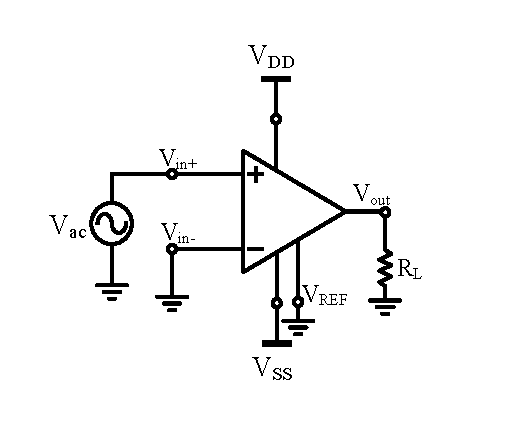
\includegraphics[scale=1]{Figures/System_Level/ahdl_OPAMP.pdf}
\caption{Behavior Modelling of Ideal OP AMP}
\label{fig:ahdlopamp}
\end{figure}

Cadence Virtuoso offers a few basic libraries and ahdllib (analog hdl library) is one of them. The ahdllib offers an ideal op amp which can used for behavior modelling to sweep gain, unity bandwidth, input impedance, and slew rate. The test setup for this modelling is as shown in Figure.\ref{fig:ahdlopamp}. The $V_{REF}$ reference voltage is typically used to set the DC level of the OP AMP. Generally, the middle voltage between $V_{DD}$ and $V_{SS}$ is the value set for $V_{REF}$. And in this case, as we have a dual bipolar supply, the $V_{REF}$ is grounded. The other behavioral inputs to these are the open loop gain, unity gain bandwidth, input impedance, output impedance, bias current, slew rate, maximum output current. The open loop gain, unity gain bandwidth, slew rate are swept over a wide range of values with input impedance a value much higher than the output impedance of the OTA. The bias current is set to zero and the maximum output current is left unset. The OTA designed is cascaded with the ideal OP AMP by connecting the output pin of the OTA to the non-inverting terminal of the ideal OP AMP. The unity gain bandwidth of the OP AMP that provides the overall system bandwidth that matches the specification is is the unity bandwidth with which the OP AMP has to be designed. And likewise, the value of gain that stabilizes the overall system is the open loop gain of the op amp to be designed. Following the steps above, the specifications of the OP AMP to be designed are tabulated  below.

\begin{table} [H]
\centering
\begin{tabular}{@{}cc@{}}
\toprule
Parameter					& Value				\\ \midrule
Open Loop Gain				& 30 dB				\\
Gain Bandwidth Product		& 6 MHz				\\
ICMR (min)					& -1.85 V			\\
ICMR (max)					& 1.2 V				\\
Output Voltage Swing		& -2 .. 2 			\\
Slew Rate					& 900 V/us			\\
Input Impedance				& 10 M$\Omega$		\\
Output Impedance			& 55 K$\Omega$		\\
\bottomrule
\end{tabular}
\caption{Specifications of the OPAMP to be designed}
\label{tab:OPAMP_Specs}
\end{table}

The two-stage circuit architecture has historically been the most popular approach to op amp design. The main reason for that being it can provides a very high gain and a high output swing. The two stages refer to the number of gain stages in the op amp. An optional output buffer to the op amp can be used as a third stage. 

Optimal compensation of op amps are arguably one of the most difficult parts of a design. Two most popular approaches are dominant pole compensation and lead compensation. Compensation capacitor between the output of the gain stages causes pole-splitting and achieves dominant pole compensation. This capacitor is known as Miller capacitor and the op amp is called as a two stage Miller compensation op amp. With the use of this compensation capacitor, the location of the poles can be chosen and thereby the bandwidth of the op amp can be set according to our requirements. This is important because the we need a 6MHz unity gain bandwidth from the OP AMP to meet our requirements and to get a stable enough system.

\subsection{Schematic}
The schematic of the Miller compensation op amp is as shown in the Figure.\ref{fig:OPAMP_Schematic}. The bias current to the differential pair is provided through the current mirror pair of $M_5$ and $M_8$. The bias current is controlled through the transistor $M_9$ whose gate voltage is provided by the voltage divider formed by the resistors $R_{b1}$ and $R_{b2}$. $C_C$ is the compensation capacitance between the two stages of the amplifier.
\begin{figure} [H]
\centering
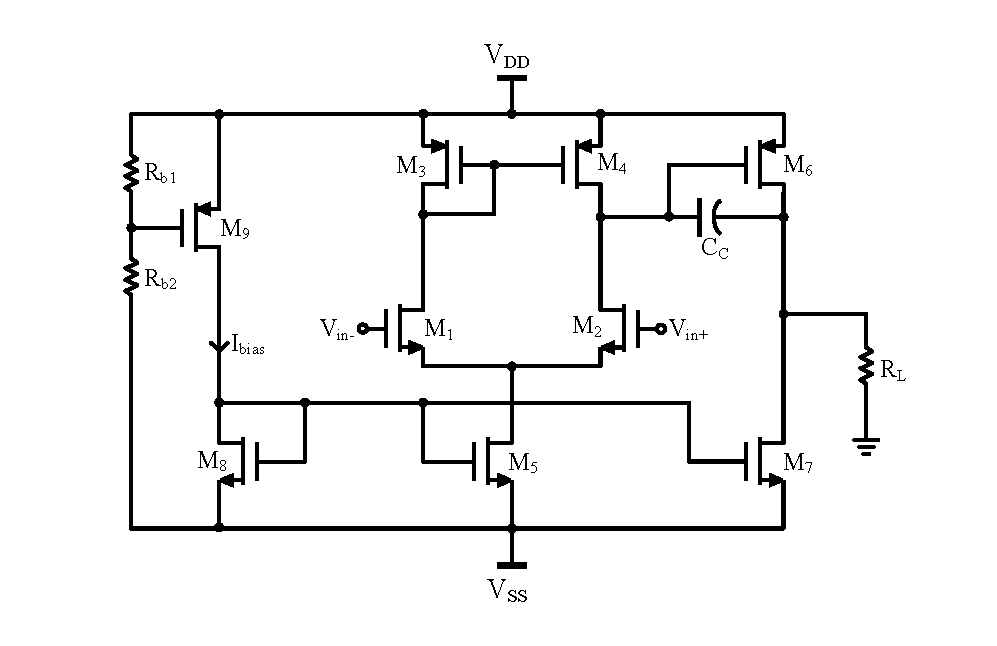
\includegraphics[scale=1]{Figures/Schematics/OPAMP_Vbias.pdf}
\caption{Schematic of the OPAMP Designed}
\label{fig:OPAMP_Schematic}
\end{figure}

The dimensions of the transistors are tabulated in Table.\ref{tab:OPAMP_dimensions}. One can easily recognize that the transistors at the output are large. This is designed so to make sure the op amp provides a very high current and thereby avoiding a common collector amplifier at the output of the op amp to amplify the output current. The compensation capacitance value is 50fF.

\begin{table} [H]
\centering
\begin{tabular}{@{}cccc@{}}
\toprule
Transistor			& Width				& Length			& Multiplier \\ \midrule
M1					& 5u				& 500n				& 2			\\
M2					& 5u				& 500n				& 2			\\ 
M3					& 30u				& 500n				& 1			\\
M4					& 30u				& 500n				& 1			\\ 
M5					& 2u				& 500n				& 1			\\
M6					& 85u				& 500n				& 55		\\ 
M7					& 50u				& 500n				& 48		\\
M8					& 2u				& 500n				& 1			\\ 
M9					& 700n				& 500n				& 1			\\
\bottomrule
\end{tabular}
\caption{Dimensions of the Transistors of the designed OPAMP}
\label{tab:OPAMP_dimensions}
\end{table}

\section{Test Setup}

\begin{figure} [H]
\centering
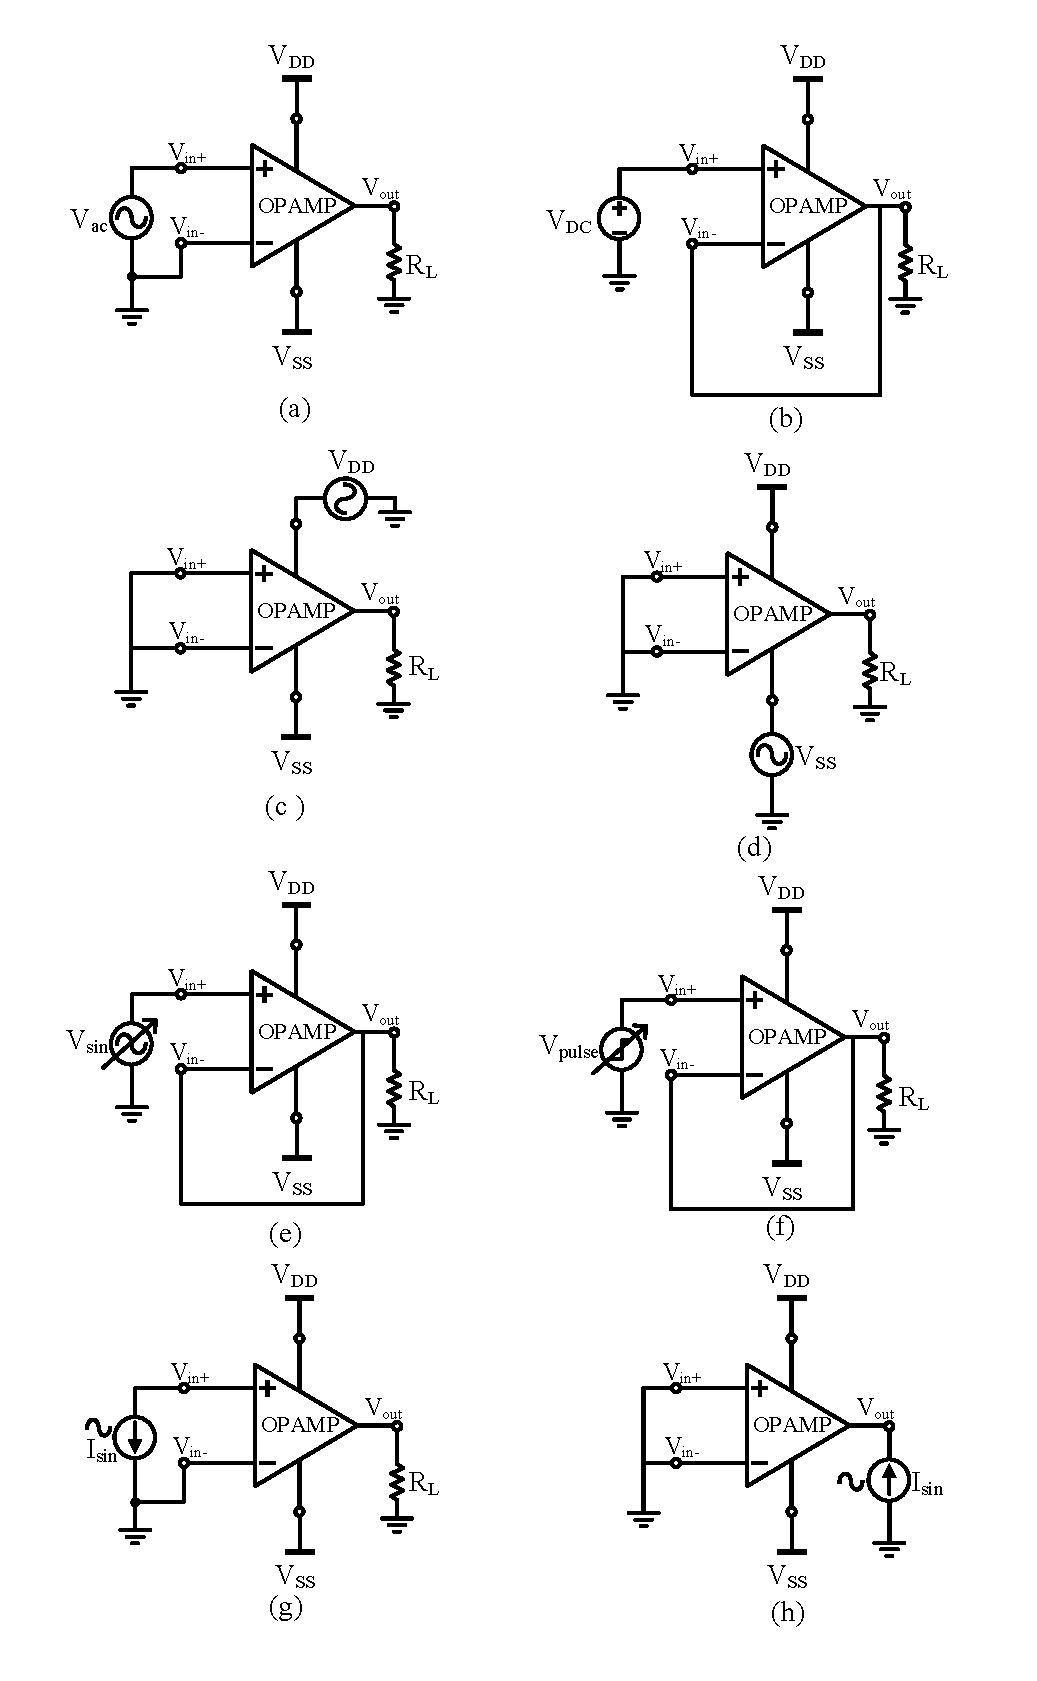
\includegraphics[scale=0.8]{Figures/Test_Benches/OPAMP_TB.pdf}
\caption{Test bench setup for OP AMP}
\label{fig:OPAMP_TB}
\end{figure}

\subsubsection{DC Analysis}


\subsubsection{AC Analysis}
The open loop gain and the gain bandwidth product are inarguably the most important parameters of an operational amplifier. Before the op amp was actually designed, these parameters were simulated with the help of an ideal op amp from the ahdlLib in Cadence. In order to have a stable system, i.e., an OTA with an OP AMP buffer in a cascade configuration, it is necessary to have the dominant poles far from each other. So that is the reason for the OTA to have a high bandwidth and correspondingly the OP AMP bandwidth can be adjusted so as to reach the specification and also to have a stable system.

The test bench used to measure these parameters is as shown in Figure.(a). The op amp is configured in an open loop. The DC biasing to the differential transistor pair is provided by the output of the OTA, which is centred around 0V. 

$V_{DD}$ = 2.5V; $V_{SS}$ = -2.5V; $V_{ac} magnitude $ = 1 V; $R_L$ = 50$\Omega$.

The plot of the open loop gain and the phase of the op amp is as shown in the Figure.\ref{fig:OPAMP_gain_pm_gbw}. The open loop gain of the op amp is 30.8dB. The gain bandwidth product is 6.2MHz and correspondingly the phase margin is $76.79^0$.

\begin{figure} [H]
\centering
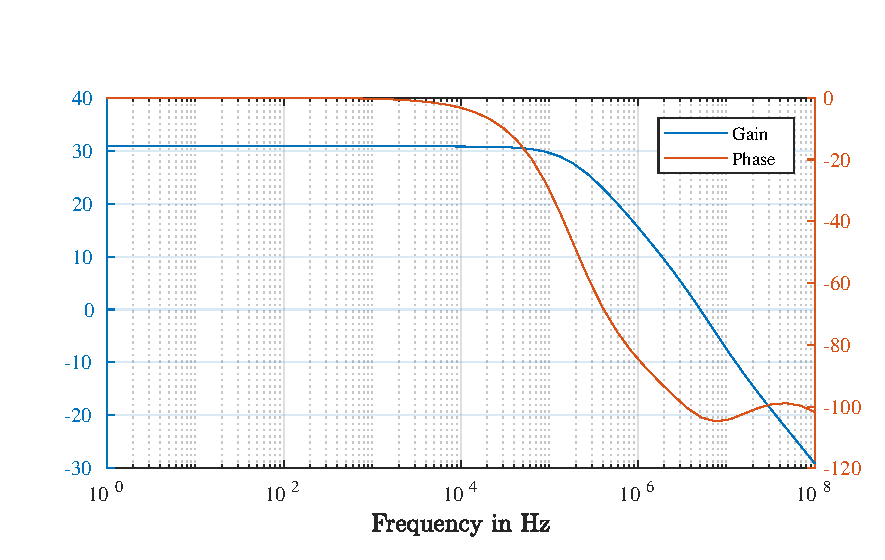
\includegraphics[scale=1]{Figures/Plots/OPAMP_Gain_PM.pdf}
\caption{OPAMP Plot of Gain and Phase vs Frequency}
\label{fig:OPAMP_gain_pm_gbw}
\end{figure}

The PSRR of the OTA in the first stage was in the range of $nA/V$ and hence neglibigle. However, the op amp designed exhibits a relatively high value of PSRR. This is due to the bulky transistors at the output stage. The test bench to measure the PSRR of the op amp is as shown in the Figure.(c). The one on the left is used to measure PSRR for a change in $V_{DD}$. And similarly, the one on the right side is used to measure PSRR for a change in $V_{SS}$.

$V_{DD}$ = 2.5V; $V_{SS}$ = -2.5V; $V_{ac} magnitude $ = 1 V; $R_L$ = 50$\Omega$.

The PSRR ($V_{DD}$) of the op amp is 30.96 uA/V, and PSRR ($V_{SS}$) is 130.96 uA/V. In the next chapter, it is seen that the assymetry in the two PSRR values doesn't affect the PSRR of the whole system.

The test bench to calculate the input impedance follows a similar concept to that of the OTA. i.e., a unity current source is connected to the non-inverting terminal of the op amp and the voltage at that terminal is measured which in turn is the magnitude of the input impedance of the op amp.

To have a stable system, it is important that input impedance of the second stage is higher than the output impedance of the first stage. Given that the output impedance of the OTA is generally high, the input impedance of the op amp becomes a very important parameter. And th input impedance is found to be 9.04M$\Omega$.

$V_{DD}$ = 2.5V; $V_{SS}$ = -2.5V; $I_{sin} magnitude $ = 1A.

Op amps are known to have zero or very low output impedance. Along with this theoretical fact, the op amp in this work is designed to retrieve very high currents, so it is expected to have a very low output impedance. The value of the output impedance is observed to be 4.167$\Omega$.

\subsubsection{Transient Analysis}
The test bench to perform the transient analysis is as shown in the Figure.(e). The op amp is connected in a negative feedback configuration so as to analyse its behavior as a voltage buffer.

$V_{DD}$ = 2.5V; $V_{SS}$ = -2.5V; $V_{sin} amplitude $ = 1.5V; $frequency$ = 1MHz; $R_L$ = 50$\Omega$.

The of input voltage and output voltage with respect to time is as shown in the Figure.\ref{fig:OPAMP_Vout}. The output follows the input only with a very small delay.

\begin{figure} [H]
\centering
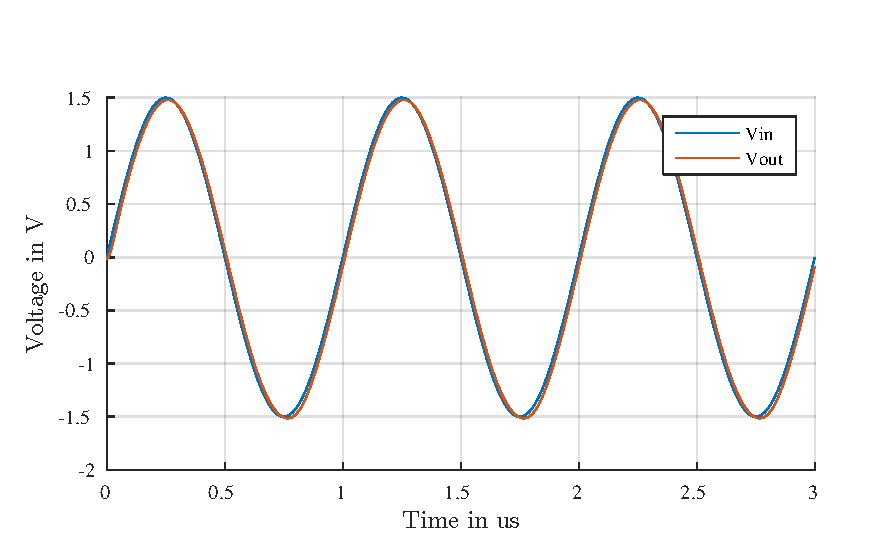
\includegraphics[scale=1]{Figures/Plots/OPAMP_Buffer.pdf}
\caption{OPAMP Plot of Output Voltage vs time}
\label{fig:OPAMP_Vout}
\end{figure}

The output current of the op amp is effectively the current flowing through the load resistor $R_L$. The plot of current versus time is as shown in the Figure.\ref{fig:OPAMP_Iout}. The current is $180^0$ out of phase with the voltage and it ranges from -30mA to 30mA for a 50$\Omega$ load and 3V peak to peak input voltage. 

\begin{figure} [H]
\centering
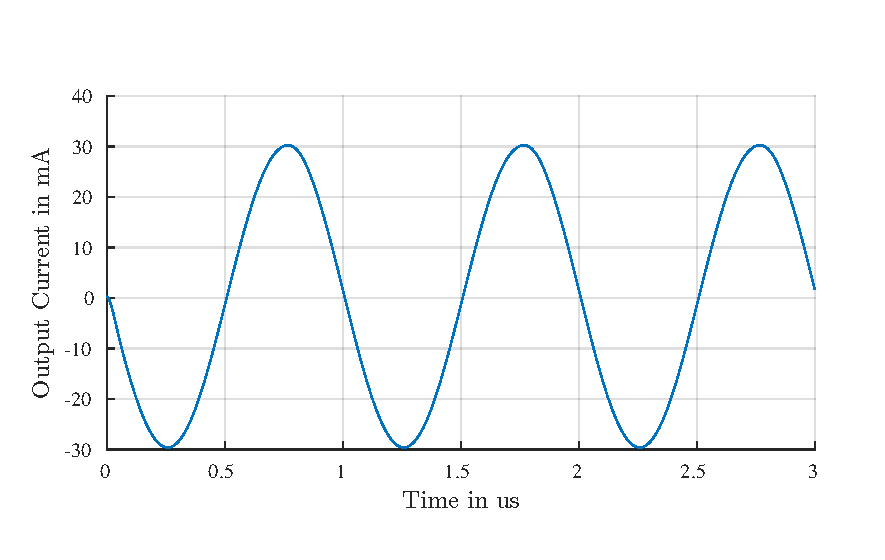
\includegraphics[scale=1]{Figures/Plots/OPAMP_Iout.pdf}
\caption{OPAMP Plot of Ourput Current vs time}
\label{fig:OPAMP_Iout}
\end{figure}

\section{Summary}

The values of all the parameters of the op amp discussed so far have been tabulated in Table.\ref{tab:OPAMP_Results}
\begin{table} [H]
\centering
\begin{tabular}{@{}cc@{}}
\toprule
Parameter					& Value				\\ \midrule
Open Loop Gain				& 30.8 dB			\\
Gain Bandwidth Product		& 6.2 MHz			\\
Phase Margin				& 76.79				\\
ICMR (min)					& -2.19 V			\\
ICMR (max)					& 2.089 V			\\
Output Current (max)		& -29.6 mA			\\
Output Current (min)		& 30.28 mA			\\
Output Voltage Swing		& -2.19 .. 2.323 	\\
Slew Rate					& 10 V/us			\\
PSRR (VDD)					& 30.96 uA/V		\\
PSRR (VSS)					& 138.8 uA/V		\\
Input Impedance				& 9.04 MOhms		\\
Output Impedance			& 4.167 Ohms		\\
\bottomrule
\end{tabular}
\caption{Simlation Results of the OPAMP}
\label{tab:OPAMP_Results}
\end{table}